\chapter{Learning from Ethics in Dementia Research}
\label{EthicsChapter}

\section{Introduction}
\label{Ethics:Intro}
In this chapter, I present insights into the ethical experiences and practices in the field of HCI and dementia, where I interviewed 22 researchers from diverse countries, institutions, and disciplines. As the previous chapters have explored the involvement of people with dementia, students (designers/developers), this chapter examines the insights strictly from the researchers perspective of their own cultivated practices. While exploring researchers concerns of participatory approaches in this line of work resonated in chapter four, many conversations I had with dementia researchers at HCI conferences sparked interest in collaborating on this particular project. 

A version of this chapter was published at CHI'20 \citep{hodge_relational_2020} with collaboration from  Dr. Sarah Foley, Dr. Rens Brankaert, Dr. Gail Kenning, Dr. Amanda Lazar, Dr. Jennifer Boger, and Dr. Kellie Morrissey. In this study, I was responsible for methodology, data collection, data analysis, leading the study, and writing the paper. While I directed the study, the paper is highly collaborative and it must be acknowledged that many of the authors influenced the ideas and arguments of the paper. With this in mind, I revisited the study and expanded the discussion section to a) fit with the thesis themes, and b) to ensure the contribution in the thesis is firmly my own.

As discussed in the previous chapters, I became aware of the many difficulties of working with everyday experiences in dementia - particularly navigating ethical review boards and stakeholder relationships. From here, over 2019, I began to have  conversations with researchers (those who are authors of the paper) on their experiences of working in institutional ethics and understanding the ways to work with people with dementia. From early on, it was apparent that we had only engaged with these type of conversations through venues such as Town Halls \citep{munteanu_sigchi_2019,bruckman_cscw_2017,frauenberger_research_2017} and conference workshops at ACMvenues \citep{waycott_ethical_2015,lazar_hcixdementia_2018} and felt that coming together as a community of practice, could provide deeper insights into the complexities that are involved when conducting ethical and engaging research with people with dementia. Furthermore, several of the authors (myself included) ran a workshop centering on inclusivity, personalisation, and scalability \citep{brankaert_intersections_2019}. We ran this workshop at DIS'19 and I led some early converastions on writing a paper on ethics and dementia \ref{fig:EthicsWorkshop}. 

\begin{figure}[htp]
\centering
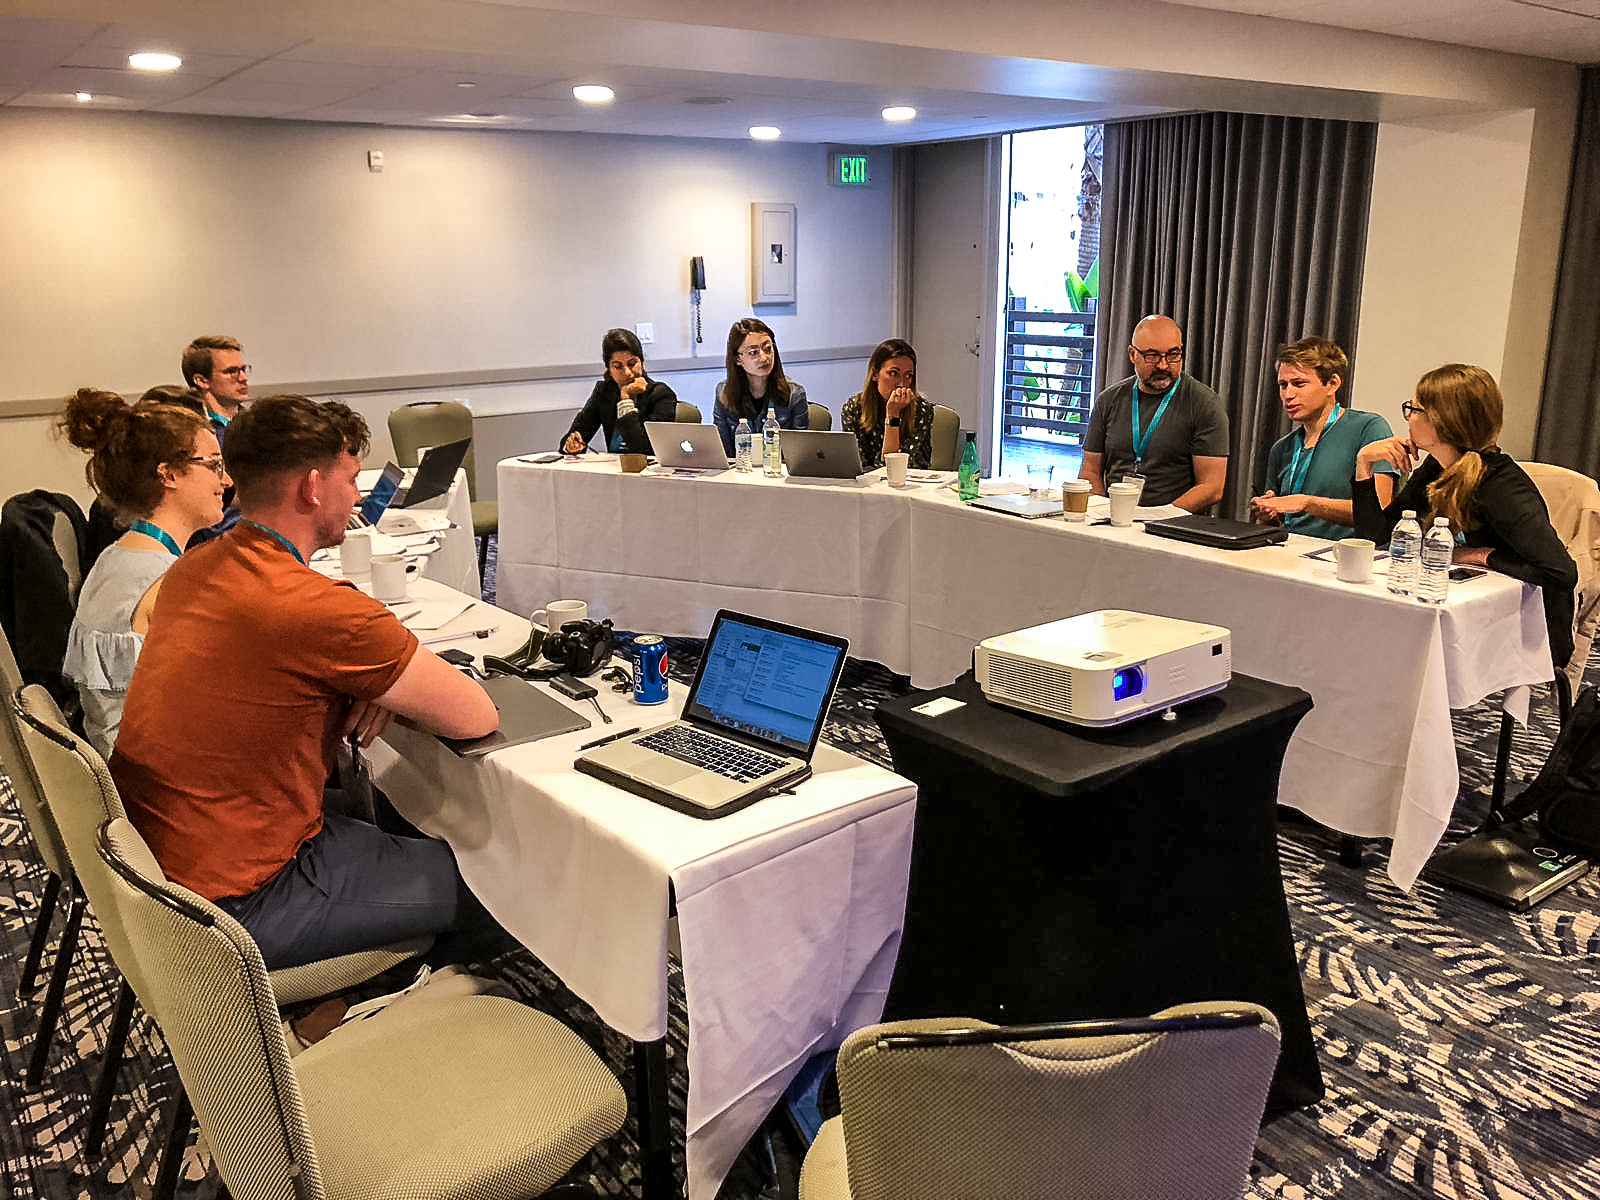
\includegraphics[width=.8\linewidth]{Images/ChapterSix/DIS_Workshop.jpg}
\caption{Workshop at DIS'19}
\label{fig:EthicsWorkshop}
\end{figure}

A particular interest has arisen in working with participants in sensitive contexts, due to the unique challenges that arise due to what it means to participate when capacity is difficult to ascertain \citep{foley_printer_2019,lazar_using_2014}, in verbal processes for people who are often not verbal \citep{knapp_nonverbal_2013,kontos_integrating_2018,john_killick_claire_craig_creativity_2012}, and recognition of participants involvement throughout the study \citep{wallace_enabling_2012-1,lindsay_empathy_2012,morrissey_creative_2015}. To date, these conversations have helped share experiences that are often based on a single research project. Yet we are missing an understanding of how researchers in a diverse array of contexts handle ethical decisions. As an example of a topic that emerged in this study through considering different viewpoints, Ethical Review Boards (ERBs) are in place to ensure research is following standard ethical principles, with the aim of protecting the participants, researchers and research institutions \citep{flicker_ethical_2007}. Despite playing a key role and coming up repeatedly in town halls in terms of questioning how the HCI community can think about ethics given the variation (or lack) of ERBs in the international context, there has been little research to date that examine the impact of ERBs on research in HCI. With this in mind, this chapter takes design ethics in dementia and HCI research as a study to reflect as a community of practice and to elucidate broader concerns about ethics in HCI research.

\section{Related work}
\label{Ethics:RelatedWork}
The following sections summarise working practices around ethics in HCI and the nature of the complexities that can arise from working with technology and design in dementia research and, more broadly, in sensitive contexts.

\subsection{Design \& ethics in HCI}
\label{RelatedWork:DesignEthics}
HCI and design researchers have long recognised the role of building relationships between the designer and the user that facilitates viewing and understanding the user is more than a test subject \citep{wright2008empathy}. Many approaches follow a similar pursuit, such as experience centred design \citep{morrissey_value_2017}, feminist HCI \citep{bardzell_towards_2011}, value-sensitive design \citep{friedman_value-sensitive_1996}, and participatory design \citep{bannon2018introduction}. Over the past decade, researchers have leveraged these participatory design methods to engage with those considered marginalised. However, as researchers have adapted ethnographic research, design probes, and co-design to fit the needs of their user populations, these practice-based methods present considerable challenges for researchers navigating through emotionally and contextually complicated researcher settings \citep{vines_configuring_2013}.

In most cases, navigating the preparation of such a study requires researchers to receive ethical approval from institutional ethical review boards who define ethical practices through a set of institutional ethical procedures. In the UK, these bodies are known as ‘Ethical Review Boards’ (ERBs) that are present across all universities and are put in place to ensure research follows sound ethical principles and puts the welfare of participants at the forefront of the research \citep{pachana_can_2014}. While most, if not all, often reflect the philosophical basis of morality, ERBs are significantly shaped by their culture and society, resulting in a vastly different set of expertise and approaches to reviewing research ethics \citep{flicker_ethical_2007}.

While these ethical guidelines set a course for research that seeks to ensure that both the participant and research institute are informed and protected, many prominent interdisciplinary research approaches, such as participatory design and qualitative work with vulnerable populations in HCI, can be considered ethically questionable ERBs. \cite{bell_censorship_2014} argues that many ERBs’ approaches to ethics align more with biomedical and experimental scientific methods, which fail to reflect the multiple ways of generating knowledge that encompass the third wave of HCI \citep{bodker_when_2006,lazar_critical_2017}. \cite{carla_introducing_2013} suggests that for qualitative researchers,\textit{ "ethical issues arise from the very beginning of the research, they stay with us throughout our interactions with our research participants, and they continue to be relevant throughout the process of dissemination of the research findings"}, and call for a prolonged and adaptable approach to ethical research design. 

For most research, these guidelines may be relatively straightforward. However, the introduction of technology may bring additional complexities concerning privacy and data storage; health and educational support \citep{gray2016inscribing}; technology longevity \citep{foley_printer_2019}, and technology responsibility \citep{ferrario_software_2014}. These challenges have been navigated and discussed in detail through ACM Town Halls and conference workshops \citep{frauenberger_research_2017,munteanu_sigchi_2019,waycott_ethical_2015}. Researchers have been invited to reflect and consider the ethical challenges they face within this space. While recent work in HCI has begun to examine the role of ethics in HCI research - particularly studies that work within sensitive settings, there is a need to come together as a community of practice to identify institutional and relational ethical challenges - in this instance, the context of dementia. As this thesis focuses on dementia, the following literature briefly introduces the current state of ethics in dementia and HCI research.

\subsection{Ethics in context: Dementia and HCI}
\label{RelatedWork:DementiaandHCI}
As described throughout this thesis, a diagnosis of dementia comes with varying cognitive changes \citep{hampson_dementia:_2016}. With dementia, the decline may change social functioning, judgement, problem-solving and may require care or other support to engage in social or complex activities. Given the vast complexities that a diagnosis presents, many of these can be seen as ethical concerns, making it a difficult space for both research and care practices. Person-centered approaches to dementia care have called attention to how we communicate with people with dementia \citep{oyebode_mental_2005}, debated the need for ongoing consent processes \citep{dewing_participatory_2007}, questioned the contested use of lies and deception in care \citep{elvish_lying_2010} and promoted the need to attune to embodied, non-verbal communication \citep{group_patron_2019,twigg_dress_2013} as key considerations in ensuring the person with dementia is respected and engaged within their own care. These practices, largely initiated within nursing and social care, have implications for research and design which seeks to work with and for people living with dementia, avoiding practices that devalue or disregard the experience of the person living with dementia. Design and technology solutions that focus on cognitive decline, monitoring and management may perpetuate stereotypes and contribute further to the stigmatisation of dementia \citep{low2020negative}. In contrast, HCI research that extends from person-centred approaches to dementia is a growing body of work that relies on relational processes as the basis of design. This has resulted in the introduction of technologies that evoke emotion \citep{wallace_enabling_2012-1,houben_foregrounding_2019,dixon_approach_2020} , engage in creativity \citep{lindsay_empathy_2012,morrissey_im_2016} and support inclusion \citep{welsh_ticket_2018,foley_printer_2019,treadaway_sensor_2016}.

Participatory and co-design projects have innovated some of the methodological approaches to design, which are necessary to support people living with dementia to engage meaningfully in co-design processes \citep{branco_personalised_2017}. This includes engaging in longer-term projects \citep{hendriks_challenges_2014}, working within the family ecology of care \citep{keady_involving_2007}, and navigating gate-keeping within institutions \citep{sanghera_methodological_2008}. The care and ethical consideration needed to include the voices of people living with dementia in HCI research has resulted in a strong relational basis for design practice \citep{bartlett_citizenship_2014,kontos_integrating_2018}. The established state-of the art based within this work has moved away from the biomedical deficit model of dementia, resulting in several underlying person-based values in design practice. This includes: treating the person living with dementia as an individual in context; including the person living with dementia in research processes that are explicitly aiming to improve their quality of life; acknowledging that dementia is a complex experience that often also includes social complexity \citep{keyes2019living}, ageing and multi-morbidities \citep{buse_materialising_2016}, which require attuning to in design and research responses. It can be argued that these design decisions offer particular ethical stances that appear essential to both the success of HCI projects in this context, and ensure the researcher-participant relationship is navigated with mutual respect and care \citep{foley_care_2019}. Making these ethical decision-making processes more visible within our empirical work has the potential to critically inform the current institutional and relational ethical framing in which we currently work \citep{oyebode_mental_2005}, and make more apparent considerations needed to ensure meaningful and engaged research with vulnerable user groups is central to the design of technologies and systems. 

However, even as these views of dementia evolve in research and practice, research shows that work in sensitive settings such as dementia can raise concern from Ethical Review Boards (ERBs). \cite{pachana_can_2014} further highlight that committees may be \textit{“subject to the same biases and stereotypes present in the general population”}. ERBs unaware of such biases may focus on the aims of protection instead of the approval of research that attends to topics such as agency and ensures meaningful participation. Further complexity arises since ERB decisions vary even within the same country or region \citep{edwards_research_2004}. This is because the decisions and reasonings are made at a university level and influenced by cultural and local norms and customs. Thus, the disciplinary changes in working with populations such as dementia are not necessarily matched at the level of those who make decisions about what research is and is not allowed when carrying out participatory work with participants who are considered ‘vulnerable’, this tension is a key focus that we attend to in this study.

To understand ethical experiences and practices in the field of HCI and dementia, I interviewed 22 researchers from diverse countries, institutions, and disciplines. Our analysis uncovers tensions arising from institutional ethical practices in socially oriented research. While ERBs vary significantly in their cultural and disciplinary approaches to dementia research, the findings reveal the tensions that arise in participatory research due to ERBs’ tending to focus on protecting participants, which raises concerns with acknowledging participants and building relationships. Through the interviews, researchers reflected on how ERBs could be more reflexive bodies, where researchers can seek support, guidance, and collaboration from experts. Researchers also shared insights from their own cultivated practices from establishing clear expectations for participants, knowing when and how to involve participants in the research, and appropriately acknowledging their contributions to our work. The chapter progresses from these rich findings from a growing body of work in HCI and dementia towards establishing a new set of fluid ethical practices to direct work in this ever-increasing area of socially-oriented HCI research. 

\section{Methodology}
\label{Ethics:Methodology}
Interested in the tacit and unstated practices that researchers employed in working with people with dementia and their carers, I undertook a reflective qualitative approach to carrying out this empiracal research. I invited 22 self-identified researchers and/or designers to one-to-one questions to elucidate wider concerns about ethics in HCI research. The following study tackles \textit{What are the ethical implications for people with dementia to participate in HCI research?}

\subsection{Participants and recruitment}
\label{Ethics:Participants}
I recruited 22 self-identified designers and/or researchers (12 women, 10 men). Each participant reported significant experience in working with people with dementia in the design of technologies and services. Participants demographics are summarised in table \ref{Ethics:Demographics}. I approached recruitment through purposive sampling methods which moves away from random form of sampling, but rather adopts a process to \textit{"select respondents that are most likely to yield appropriate and useful information}(pg.317)\citep{kelly2010qualitative}. To begin with, I selected presenters, exhibitors and attendees from Dementia Lab conferences (2016-2019) - this is an international conference featuring design and HCI work with people with dementia \citep{brankaert_dementia_2019}. Once participants from Dementia Lab expressed interested, I employed snowball sampling, which asks current participants to recommend potential participants of interest who have similar experiences to design, HCI and dementia \citep{noy_sampling_2008}. In the demographic table, participants were asked to self identify their career stages as: early - junior researcher/lecturer, mid - senior researcher/lecturer and senior - professor.

% Please add the following required packages to your document preamble:
% \usepackage{graphicx}
\begin{table}[htp]
\centering
\resizebox{\textwidth}{!}{%
\begin{tabular}{c|cccc}
\textbf{Name} & \textbf{Discipline} & \textbf{Career Stage} & \textbf{Gender} & \textbf{Place of Practice} \\ \hline
Emily & Design & Mid & F & UK \\
Verna & HCI & Early & F & Singapore \\
Neville & Design & Early & M & The Netherlands \\
Louise & Psychology & Early & F & Ireland \\
Sofià & Design & Early & F & The Netherlands \\
Isla & Psychology & Early & F & Ireland \\
Martin & Computer Science & Student & M & United Kingdom \\
Niamh & Speech \& Language & Early & F & United Kingdom \\
Kevin & Computer Science & Senior & M & United Kingdom \\
Lucas & Computer Science & Mid & M & United Kingdom \\
Micheal & Psychology & Senior & M & Ireland \\
Jessica & Informatics & Early & F & USA \\
Daisy & Design & Mid & F & United Kingdom \\
Beth & Social Science & Early & F & United Kingdom \\
Enzio & Design & Early & M & Belgium \\
Mary & Design & Early & F & Belgium \\
Holly & Design & Student & F & The Netherlands \\
Dion & Design & Student & M & The Netherlands \\
Thomas & Computer Science & Junior Developer & M & Sweden \\
Jarod & Computer Science & Junior Developer & M & United Kingdom \\
Lisa & Computer Science & Mid & F & Canada \\
Katie & HCI & Mid & F & Australia
\end{tabular}%
}
\caption{Participant demographics}
\label{Ethics:Demographics}
\end{table}

\subsection{Ethics}
\label{Ethics:Ethics}
Newcastle University granted ethical approval for this study. Each participant was emailed an overview of what would be expected from the interview and the study, and provided with consent form and information sheets. Due to the sensitivity of the topics discussed in the interview, all participants have been anonymised for privacy purposes.

\subsection{Data collection}
\label{Ethics:dataCollection}
Mindful that the interviews would be touching on sensitive topics, I adopted the reflexive position of 'connected knowing', which involves empathy, and perspective-taking to understand the other's perspective that further recognises disagreement or disparity \citep{belenky_womens_1986}. With this in mind, while I conducted the majority of the interviews, specific interviews where the participant had a prior relationship with other authors of the study led the interview to provide a more comfortable space for sharing personal stories on dementia. For all interviews, I developed a semi-structured interview schedule (see appendix \ref{app:EthicInterview}), which consisted of open-ended questions and prompts on: 1) experience in dementia research, 2) power relationships, 3) experiences with institutional ethics processes, 4) HCI ethics, 5) building relationships with people with dementia, 6) dissemination of knowledge, 7) exit strategies, and 8) how we define impact. Interviews lasted from 45 minutes to 70 minutes. Interviews were carried out in person where possible, but were otherwise carried out over video calls. All the interviews were audio-recorded and transcribed in full.

\subsection{Data and analysis}
\label{Ethics:Analysis}
Data collection consisted of 1100 minutes (average 50 minutes per interview) stretching across 22 interviews. With the large dataset, Dr. Kellie Morrissey and Dr. Sarah Foley supported initial coding by coding half of the data to compare to my coding of the 22 interviews to avoid bias \citep{berends_using_2005}. Throughout the project, I led weekly meetings with the authors to reflect on what I saw in the data, agree on codes, subcategories and the building of themes. My analytical approach followed \cite{braun_using_2006,braun_one_2020} Thematic Analysis (TA). This process followed a seven step process. First, I prepared the transcripts. Second, myself and the other two coders familiarised ourselves with the data and referring to the research questions. Third, I began to generate labels to identify relevant data - for example, \textit{explaining the use of data'}
, \textit{'learning by observing'}, and \textit{'novelty not always necessary'}. For consistency and avoid bias, I then compared my coding with the other two authors to ensure sufficient concordance. In the fourth and fifth steps, I invited authors to take part in a Skype call to organise codes into potential themes to gain multiple perspectives and have opportunities to address disagreements and reflect on the themes that had been generated throughout the analysis. In the sixth step, I began to frame the themes around the research question and defined and named the themes. Finally, the seventh step is the developing and writing of the analysis that is presenting in the following section below.

\section{Findings}
\label{Ethics:Findings}
The findings centre around two more prominent, overarching themes that describe researchers’ reflections on ethical dilemmas and emergent practices in their research within the subthemes. The first theme considers the tension between guidelines and situated practice that highlights institutional protection and ways (or the lack of) to acknowledge the person with dementia. The second theme, emotion and everyday experiences, explores the relationships researchers co-create with participants and how researchers initiate and maintain relational approaches. Throughout the findings, I refer to the participants as researchers, as they all engage in research to one degree or another.

\subsection{Guidelines vs situated practice}
\label{Ethics:ThemeOne}
Researching under a culture of ethical ‘protectionism’ caused significant tension when working in socially-oriented research, which the participants described as requiring significantly more flexibility. To this point, the following subthemes describe the ethical challenges researchers face, including a sense of over-protection of participants, a lack of practical guidance from ethical review boards as to how to navigate ongoing ethical challenges through the research, and the effect misrepresentation of dementia has in the public eye.

\subsubsection{The unacknowledged subjectivity of ERBs}
\label{Ethics:ThemOnePartOne}
Researchers highlighted a range of different experiences with ERBs that were tied to their geographical, cultural, and institutional contexts. Holly expressed in the Netherlands that person-centred care is recognised as standard practice providing a \textit{“easy process” }as the research is not taking a \textit{“medical direction”}. Holly continued to explain finding value in describing to ERBs why \textit{“we do person centered research”} which provided the ERB with deeper insights into dementia and provided valuable understandings for her approval application. Additionally, in the UK, Daisy describes her university ethics committee as consisting of researchers \textit{“with a track record of working with people who lack capacity”}. Furthermore, this provides a diverse and inclusive lens to provide a \textit{“good framework for the ethical consideration of involving [people who are considered maganlised] and people who lack capacity”}. 

On the other hand, Verna’s ERB in Singapore considers, as a matter of course, \textit{“technology that’s implemented into a care home to be a medical device”}. Because of this, the technology and the ethical review it is connected to is evaluated much more stringently. Verna further highlights struggles about whether \textit{“engagement activities for people living with dementia [can be considered] a medical device”}. As soon as the research is being done in a hospital setting, the ERB considered it to be a medical device - \textit{“That’s like calling a ball used in therapy a medical device”}. This miscategorisation of aesthetic or pleasurable experiences as an intervention in health or wellbeing places importance on technology as having to “make the person better” in a biomedical method.

In contrast to Daisy’s success with a working relationship with UK Ethics committee’s, Beth’s experience with UK institutional ethics has been challenged where she \textit{“felt [their] knowledge and expertise was being called into question by people that were either non-experts in the field, or that it wasn’t appropriate for them to be reviewing it”}. As such, Beth’s experiences highlight issues of where decision-making processes are made by committee members who have potential biases and stereotypes of people with dementia resulting in an inaccurate view on the study proposal. Likewise, the makeup of an ERB can also lead to a biomedical view. Michael says he found significant difficulties getting ethics approved, as his relevant Clinical Research Committee, was \textit{“run by mostly medics”}. Though ERBs try to have people with experience in particular areas, due to the specialisation of research, it is not always possible to have a committee with expertise in dementia from both a person-centered and design angle. Niamh, part of the ethics committee at her university, explains that \textit{“you do not know who is going to get your proposal”}. Perhaps because of the breadth of expertise on the committee, decisions may lack 'discernment', as ERBs are perceived as taking a \textit{“one size fits all ethics... to be obstructive”}. 

Isla reflects on ‘one size fits all ethics’ when working on an application to recruit from NHS (National Health Service, UK) care homes to take part in a low-risk, qualitative design study exploring the support of intergenerational contact between young people and people living with dementia through technology. She explains that her proposal got \textit{“bounced to the NHS ethics”} and after a considerable amount of time approval was refused. The medical ethics committee could not see the \textit{“benefits of involvement”}, but instead focused on the risks concomitant with cognitive decline, and the need for protection above inclusion. 
Researchers noted that their own experience in the area was not considered in reviews. Thomas expressed that while he thinks ERBs see \textit{“the benefit in [the research]”}, that ‘trust is lacking’ towards the researcher. 

Verna describes her collaboration with care homes as being about partnerships built from trust. Similarly, Kevin proposes that ethical review forms should create a collaborative bond between the researcher and the ethics committee. Enzio suggested that ethical approval forms should give the committee information to reassure them that the researcher has the support and knows what they are doing such as: \textit{“Is there a senior researcher? Who is the junior researcher? What’s the experience?”} Overall, our participants sought a reciprocal relationship with their ERBs. They could seek support, advice, and collaborate discursively, rather than be judged for their ethical practices or denied approval entirely after a significant amount of time and effort has been expended. Similarly, our participants also sought an equal relationship with their participants.

\subsubsection{Recognition of participants' contribution}
\label{Ethics:ThemeOnePartTwo}
Researchers placed importance on acknowledging their participants’ contributions. In his design research, Dion mentioned a lack of recognition from other researchers that caused a domino effect, putting participants off from taking part: \textit{“I noticed there was this kind of, almost fatigue [from the carers], that they have seen all these researchers come by, especially many students who make these prototypes. They test it, it is all nice...but then they disappear. There is nothing that remains.” }
When Dion explained his research to the participants, the participants said \textit{“Why do we need this? Why can’t there be something that stays?”} This illustrates the importance of clearly articulating what participants should expect throughout the study and acknowledging their participation in an appropriate and meaningful way. 

Katie and other’s emphasised designing research to be \textit{“engaging, enjoyable and rewarding”} for the participants as a way to a) recognise the \textit{“time they are giving up”} and b) to provide a \textit{“space for creativity and sharing”}. Beth reflects on one participant who said:

\begin{quote}
\textit{     “you know, this has been so amazing [to be part of the research] because actually, we never got any information when we got the diagnosis and we have no one to talk to, nowhere to go, and it has been so lovely just having a conversation”. 
}
\end{quote}

As such, while Beth describes that for many who have felt shut out from a diagnosis, that research offers an opportunity for people with dementia to talk to experts who may know where to find resources and offer alternative directions for the person with dementia to find ways to take part int he community. Similarly, Martin comments on how participants would express to be “\textit{part of future studies”} and that they were \textit{“extremely thankful to be listened to and to be listened to again”}. Where many people with dementia often express difficulties in participating in society post-diagnosis \citep{bartlett_citizenship_2014}, the researcher’s illustrate the importance of recognising people with dementia's participation in research.

Typically, researchers will often pay their participants with vouchers for their time. However, Thomas stated that in care homes, money \textit{“doesn’t really work in this setting… money does not hold too much value there”}. If the traditional approach to compensation does not work in this setting, we must consider other ways to compensate people with dementia for their participation. One approach is to offer participants the technology that we build. In our conversation with Niamh, she discussed a different approach to disseminate research to be useful for the participants: \textit{“So, we co-designed a toolkit with them and left them with the toolkits and left research materials, and things, when we went over…they were really taking time out of their- you know, some of them were travelling up to three hours just to get there. Three hours, three hours back, just to come early to come and do these things.”}

Though this approach works well with some research, other HCI projects focus on initial exploration, where prototypes are not fit to withstand long time use without continuous check-ups and fixes. Echoing this, Isla shared concerns \textit{“of anxiety and failure”} if the technology would break, and conflict towards the technology \textit{“may break in a year or two.”} Another way researchers give back and recognise participants’ contributions is through ceremonies or events to commemorate and celebrate participation. Through our interviews, Louise and Daisy reflected on using the term ‘celebration’ and the act of giving as a way to value their participants work through the study. Daisy sees the celebration as \textit{“a way of celebrating the lives of the participants that have helped develop whatever you’ve found”}. Louise reflects on creating personalised gifts and celebrating research with those involved through her PhD study: \textit{“For them, maybe I just came in, but for me, it was a very meaningful relationship. I probably just didn’t want it to end, to be honest.”} Researchers need to celebrate a finished project not only for the participants but for themselves, highlighting the personal impact of this kind of research. Regardless of how we acknowledge contribution, we should recognise participants as individuals who have contributed to the research and that their knowledge, experience, and time are valuable and valued.

\subsubsection{Protection vs acknowledgement}
\label{Ethics:ThemeOnePartThree}

Keeping participants anonymous is the standard ethical practice \citep{novak_anonymity_2014}. Researchers use pseudonyms and blur faces in photographs to ensure data collected cannot be traced back to the original participants. Throughout the interviews, researchers expressed an understanding of safety and respect to the participants when anonymising data. However, Kevin noted that this approach seems to be more about "making sure we stay within the university's insurance" and less about \textit{"avoiding harm to participants"}. Similarly, Beth describes universities avoiding harm that caused additional frustrations for the research team. For instance, the team "had to ensure [transcription] was only dealt with by the research team", and the \textit{"video recording of participants"} caused a \textit{"massive problem"} with the ethics committee despite the necessities of researching \textit{"body language in dementia"}. 

Daisy mentions that anonymisation works when participants \textit{"might not want their [real] name [used]"}, but when participants want to be recognised for their contributions, challenges can arise. Several researchers commented on their challenges when participants want to be acknowledged as co-creators. Lucas reflected on previous work where he had participants ask \textit{"We have done this work… Can we have some credit for it? Can our names appear in the research?"}. But as it stands, \textit{"they can't, because [the] ethics board says it must be anonymised."} Researchers, especially in social science, endeavour to have participants real names ethically passed by the review board. Daisy highlights further tensions because of this tendency towards protection that universities exhibit when it comes to research with dementia: institution protection can further add to the feeling of "\textit{dementia rob[bing] people of their dignity, their individuality and their lived life."} Through Daisy's awareness of working with people living with dementia, she believes that \textit{"to make them then anonymous or a number is robbing them of their dignity."} Dion considers appropriate ways to acknowledge the person living with dementia's contribution through a photo shoot for a care organisation magazine: 
\begin{quote}
\textit{"[the photographer] came by to take some pictures and ask for permissions, and I was with the participant, interacting, but it was a bit fake, of course." 
}
\end{quote}

Dion reflects on this moment, saying the participant \textit{"was enjoying it"}, and was \textit{"laughing"} during the activity. The participants were particularly \textit{"proud that she could be on the pictures, and in the magazine's article"}. A growing number of publications include people with dementia as authors to recognise their contributions. 

Enzio named a UK institution that hired participants as research collaborators and, through this, ensured they were given authorship of subsequent publications: \textit{"I think this in-between solution is great. If you have a participant who is joining you for some time, [hiring] would be great to do. Then they are equal to you as an author of work or papers.}" Jessica also mentions Dementia Enquirers \textit{"who have a project where people with dementia are coming up [with research studies] and that have [their own] ethics [guidelines]."} Recognising participants by opening up authorship ensures participants are influencing the research agenda, in contrast to the current standard practice of anonymisation of participants. However, the ACM code of authorship states that authors must \textit{"have participated in drafting and/or revision of the manuscript"} \citep{noauthor_criteria_nodate}. We, therefore, need to question whether the ACM model should shift towards a contributorship model, in which contributions towards the project are credited rather than academic writing.

\subsection{Emotion and everyday experiences}
\label{Ethics:ThemePartTwo}
Through our interviews, researchers described various views on their work’s ideal and realistic impact. In this theme, we unpack the subjective role of time in research impact and the importance of building and continuing relationships that hold meaning as part of the research.

\subsubsection{Research pace and relationships}
\label{Ethics:ThemePartTwo:Time}
Researchers noted the tensions arising when the timeline of a research project does not align with researchers' best practices. There are differing views on what should be emphasised: one perspective espouses allowing relationships to develop slowly over time, while the other emphasises the value of a swift design process where visible progress is made in step with technology development. From our interviews, it was common to hear how important it was to researchers to create relationships throughout the research. Niamh mentioned times where she questioned \textit{"I wonder if this is the right time for you (the participant)"}. At odds with timelines that rush data collection for a deadline, several researchers emphasised a more relational approach that takes time and care throughout the entirety of the study, up to its ending. 

Michael comments on how researchers should be considering continuity and not be \textit{"dropping in and out of care homes or people's lives for two or three months to get data to write a paper"}. He explains that it is unreasonable \textit{"to jump into people's lives… and come back and expect them to be open-armed and welcoming us again three months later"}. In situations where this is not feasible as part of the research, Dion would often \textit{"go and meet the participants"} at the residential between studies to maintain a relationship with the care staff and residents. Similarly, Isla suggests, \textit{"go and have a coffee or work to their schedule, I guess. They are the most important part of our research."}

Consequently, the researchers expressed that through building stretched out processes, Isla argues we provide the time to \textit{"think about sustainability, scalability... and be mindful and treat every single person as a person and not racing to the finish line"}. A knock-on effect that researchers highlighted was the building of relationships outside the research scope. For instance, Louise described \textit{"personal relationships"} shaped by spending time with residents where they \textit{"could be so open"} and would be \textit{"delighted to have someone to listen to them"}. Daisy described how she felt the relationships we make in research never \textit{"stop and [we] never let go"}. Daisy continued to describe the development of \textit{"good relationships"} that would "tend to continue informally" and that while they would \textit{"contact very rarely"}, those relationships that are formed over a long period \textit{"don't stop existing"}. 

While some researchers express the need to take more time in the research process and the potential outcomes of long-term relationships forming outside the research, Lucas mentioned that design iteration is \textit{"too slow of a process"}. While he agrees relationships should take as much time as they need to develop, it should speed up once the study moves to iteration and design. Lucas continues to describe the need to move towards a \textit{"more hackathon pace"} where iteration and changes to prototypes are a "daily or weekly basis". By leveraging \textit{"wizard of OZ"} and\textit{ "lo-fi prototyping"}, people with dementia and designers can focus on the \textit{"interactions rather than designing the final systems"}. In a similar vein, Kevin emphasises the challenges technology brings when \textit{"technology just ages really quickly"}, which requires fast iteration processes to provide \textit{"top of the range technology in the area"}. 

Returning to Lucas, he describes frustration participants may experience if they are expecting something to be built: 

\begin{quote}
\textit{    "meeting and chatting with someone for a couple of hours each week can feel like not much is happening. Especially if you come back and that thing you said you would do hasn't been altered, and maybe it has to be discussed again next week". 
}
\end{quote}

Once design iteration starts, researchers should engage and involve people living with dementia in the study as much as possible and through design responses which \textit{"show people that you are taking feedback seriously}". In particular, when designing with people living with dementia, there is a distinct progression in the diagnosis over time. If we prolong the research study, \textit{"what [the person with dementia] needed at the start … might be different from what they wanted at the end of it"}. Researchers should consider how to pace the trajectory of a project, including explicitly planning for the time it takes to grow and support meaningful relationships with research participants. This is especially important with people living with dementia, as understanding each individual's communication abilities can support better engagement in research as well as better research outcomes.

\subsubsection{Understanding impact}
\label{Ethics:ThemePartTwo:Impact}
Bringing technology into research offers opportunities for meaningful engagement and ethical challenges relating to the robustness and longevity of technology when the project ends. In our interviews, researchers offered different perspectives on what is most important: the technology itself working, or the meaning and the relationships that they engender. Dion notes that it is \textit{“difficult to do these long-term solutions”}, and while it is easy to say \textit{“We need to leave something behind”}, the technology still needs \textit{“technical support.. because they break down every week or so.”} Isla reflects on a colleague who had difficulties maintaining technology after the study had ended. The researcher \textit{“guaranteed [the device] to last for the year of the study.. and will fix it [throughout the year]”}. While the researcher appropriately managed expectations of the study with participants, “\textit{one of the participants hung on to the technology for years and found it was helping [her quality of life]”}. As it broke, the participant asked for help to fix it, but “the research was gone. The funding was gone.” As researchers, Isla suggests we have a responsibility to anticipate and be \textit{“upfront and say there is a natural lifespan to some of these technologies”}. One direction researchers take is by thinking about longevity in ways other than the lifespan of the technology itself. Thomas highlights how the value in participants taking part in the research is the opportunity to have a say\textit{ “on the new social direction of that [community]}”.

In her research, Emily expresses building a sense of media’s lifespan or other possible technologies. The couple she worked with, \textit{“had pictures of things they made together [throughout the research]...and that meant a lot.”} By placing her participants as the focal point who drove the research, it became a significant event for them. Emily remarks that technology \textit{“doesn’t have to be cutting edge to be meaningful, and to do something poetic and powerful”.} In this way, it’s clear that researchers should consider that technology alone does not hold any value; it’s the relationships and experiences it creates. However, there can be an expectation of, and value, associated with longevity. Martin shared a story about his Grandad designing gifts for his Grandma:
\begin{quote}
\textit{“My Grandma looked after my grandpa through his dementia until he sadly passed away. During those years, he expressed himself creatively and would create gifts for my grandma. One Christmas, he created a beautiful Nativity scene. On the backdrop was LED lights that resembled the stars and was powered by a battery. On the back of the nativity scene, my grandpa wrote: “My love lasts as long as the battery”.}
\end{quote}

Every year, Martin’s Grandma brings out the scene for a few days and places the very same battery that she has had for over 20 years to see if it still works (\textit{“to this day, it still does”}). Kevin expressed ethical value in working with businesses to help maintain a product after the end of a project. Kevin says \textit{“grants only ever get you so far… [researchers] have got to come up with a value proposition”}. Researchers can find ways to \textit{“reinvest [money into the product] and keep the stuff going”} by bringing in businesses. Having businesses continue supporting systems and technology after the end of a study can ethically support the participants who have been part of the research and are using the technology that may have improved their quality of life. Within these more extensive projects, more comprehensive sets of skills were implicated, involving complexities on their own. Kevin iterates by working with \textit{“business people, venture capitalists”}, his study has the opportunity to find the best way for technology to get to the market, where, ostensibly, it will find further impact. Kevin further expresses that research should aim to \textit{“build robust software that can result in spin-offs or commercial partnerships to get to the next stage”}. However, this can be a contested space with participants, particularly carers, concerning how long it takes for design products to arrive on the market. This further highlights the need for setting clear expectations for participants and being responsive to the many reasons as to why they agree to partake in the design research process. 

\subsubsection{Ecology of self(care)}
\label{Ethics:ThemePartTwo:Care}
Our interviews saw several researchers talking about their emotions and how they influenced their experiences in their projects. Our interview with Enzio indicated that \textit{“building relationships between researchers and participants help to appropriate the technology around the person living with dementia and their ecology of care”}. Working primarily with students, their emotions influenced the way they formed relationships and engaged with the research. Seeing his students sensitively attending to lived experience, Enzio realised that \textit{“this would not have happened if they just made something for a generic person with dementia without having this personal relationship”}. 

Louise, who works on a study in a care home, reflected on learning from a caregivers experience. Over five years, Louise talks about one participant who “\textit{used to be engaged”}. Over time, as \textit{“her dementia progressed”}, that participant became \textit{“very shy”}. That change in personality and expression gave Louise \textit{“the best sense of what it might be like to watch a loved one in that process and try to bring them back.”} While focused on a caregiver’s lived experience, it changed Louise’s view of\textit{ “being quite critical”} of people trying to ‘bring back’ their loved one’s memory. Having spent more time on the project, Louise had a more in-depth understanding of \textit{“how it can be really difficult”} to see someone go through a diagnosis of dementia. Louise’s experience of ‘unexpected’ emotion is reflected as emotionally significant. As researchers, we have \textit{“the luxury”} to reflect on the lived experiences we are a part of. Having space and time to reflect allows researchers to understand the emotional nature of the work we are doing; Of course, working in dementia care comes with complexities in that participants may pass away, or that their dementia will likely progress. Katie expresses that this can represent \textit{“big emotional stress for researchers”}. Dion highlights the ethical and moral complexities of \textit{“hav[ing] observational data”} from a participant who had passed away before any publication. 

Similar to many other academics, Dion echoed the struggles of what to do in this situation: \textit{“Do you use the data or not? How do you mention this in a paper? Those are things that I don’t know how to handle actually. I found it very difficult. What do you do with it?”} In this instance, Dion particularly struggles between his emotions influencing his choice on whether his work be published. However, it is likely that simply not talking about the work will not divert the conflicted emotions stemming from having carried out the research in question \citep{wacquant_for_2015}. If we are moving towards reflexive practises in HCI, these seemingly personal experiences from researchers should be integrated into the empirical nature of our work \citep{morrissey_value_2017}. However, self-care is similarly important: Mary recommends to “be true to your personality and feelings” and to make \textit{“time to talk about the experience, even if this [has] no specific function in the research”}. Researchers should take time to reflect and discuss the experiences they have had through their research; in doing this, they may lay down healthier, more open and more empathetic practices for researchers who may follow in their shoes.

Through my analysis, I unpacked tensions that arise using institutional ethical practices in socially oriented research. With the importance of creating meaningful relationships, our analysis highlights the importance of recognising participants, valuing their time, and the continued ethical challenges of acknowledging people living with dementia in research. ERBs continue to over-protect participants, causing researchers difficulties of involving participants throughout a research study, including not being acknowledged for their contributions. While we are working in ‘sensitive settings’, this does not change our morality or our capacity to empathise and sympathise with other humans. Isla remarks, \textit{“we should be as present as possible...the more open and almost kind and loving you can be towards someone, the better, without compromising your self-care”}. Bringing this element to the forefront of ethical design practices may be essential in moving this research space forward.

\section{Discussion}
\label{Ethics:Discussion}
The findings indicate that ethical tensions arise when researchers find themselves conflicted between the ethical guidelines they need to comply to and the specifics of the research, such as participant characteristics, relationships that have developed over the course of the study, the role technology has taken in the participants’ lives, and the researchers’ own definition and understanding of what it means to have long lasting impact \citep{mattsson_praxisrelated_2007}. I described how researchers ethically navigate the contrast between ethics in theory and practice, ultimately requiring an ‘in the moment’ investment in the integrity of the relationship with both participants and backing institutions. Below, we discuss how our findings add to and contrast with previous work in this field and suggest future directions for HCI researchers.
Participants discussed challenges in maintaining boundaries in participant-researcher relationships. Working within an experience-centred design framework, \cite{balaam_emotion_2019} note the need for designers and researchers to be more accepting of how we engage and manage emotion in the work. Through engaging with emotion, we must consider boundaries as subjectively based on contextual knowledge of the research relationships. From the reflections presented in the findings, it is evident that emotion is an integral part of much socially-oriented HCI research, and thus must also be taken into account in considering ethics. With this in mind, the following three subsections suggest a set of future directions guided by the researchers' reflections on working with people with dementia.  

\subsection{What can researcher's and ERB's do?}
\label{Ethics:WhatCanWeDo}
From the findings, the researchers desired reflexivity in the ethical review process, where researchers can seek support, advice, and collaborate discursively. Researchers have much to communicate back to ERBs in terms of how to ensure the inclusion of vulnerable populations, which past research has argued is an ethical and moral design outcome to strive for \citep{scanlon_what_1998}.By clarifying expectations for participants, and knowing when and how to involve participants in the research, we can support better engagement in research as well as better research outcomes. However,the emotionally engaging nature of this work and empathetic response evident in the findings suggests the importance of supporting care practices - self-care and otherwise - as part of the research design. In table \ref{tab:ethicRecommendations}, I have presented a series of suggestions for ERBs and researchers to improve the relationship and processes that often structure our work.


\begin{table}[ht]
\renewcommand{\arraystretch}{1.7}
\centering
\begin{tabular}{p{0.5\linewidth} | p{0.5\linewidth}}
\textbf{Recommendations for academic ERBs} &
  \textbf{Recommendations for researchers} \\ \hline
Create relationships with community advisory groups to gain insight into population needs (also see next discussion subsection). &
  Develop specialised educational programmes that can be shared to ERBs and other researchers in the field. The programmes could consist of examples of consent/information forms, internal ethics procedures, websites/organisations that may provide support. \\ \hline
Introduce staged review processes to provide feedback and understanding for researchers to provide clarity to any ERBs potential concerns. &
Link-up community experts with ERBs to provide additional insight into an area that the ERB may be lacking expertise. \\ \hline
Consider workshops / on-call queries to provide education to researchers and the community. &
Volunteer to work for your ERB to make necessary changes from the inside. \\ \hline
Be open to learn new insights into the different everyday ethical practices researchers may require to use for the community they are working with. &
Educate the community about ERB processes and the benefits of research, and ensure the community receives actionable insights that could be implemented into their practice. \\ \hline
Consider procedures and processes that take into account the researchers' wellbeing. &
  Discuss compensation and acknowledgement to your participants to ensure they are recognised for their contribution to the research. \\ \hline
\end{tabular}
\caption{Recommendations for ERBs and researchers for ethical research}
\label{tab:ethicRecommendations}
\end{table}


\subsection{Designing for peer-led research}
\label{Discussion:PeerLedResearch}
Researchers felt that the institutional ethical application process needs to be developed further - particularly where it does not acknowledge how valuable expert knowledge from the user domain can be. This poses the question: \textit{How can research design be rooted in participant-led agendas?} From the findings, all researchers expressed the value in working with people with dementia for their experience and knowledge in the same way you would work with developers to learn about developer workflows. In all the examples within the findings, researchers highlighted various forms of compensation from monetary value, gift-giving, pleasant research activities, and contributing to the authorship of an academic publication. However, as Martin described, \textit{"many of these compensations still [present] problems of addressing power imbalanced between the research and the participants"}. With this in mind, as researchers, we must consider ways to use academic resources to centre the community to address the issues that HCI research can assist with.

For instance, \cite{reuter_older_2019} work, which made use of the university resources that are often rich in  (e.g., technical competence, A/V equipment) to innovate within a radio programme for older people, leading them to encourage researchers ‘to consider participatory action research as a method of assistance in itself, complemented by technical innovation to facilitate processes in this space. Building on her work, Reuter continued to centre the radio programmes needs by supporting grant and internal university funding as a procedure to ensure that the institution and the radio programme maintain a relationship once the researchers step away from the project \citep{reuter2021content}. 

Additionally, to provide more ethical research studies and to engage with communities from the start of the research journey, in our findings, Jessica discussed, engaging with advocates outside of HCI, such as the Dementia Enquirers \cite{davies2021dementia} , ensures that research agendas are more closely aligned with the needs of the population, thus \textit{“helping improve the quality, relevance and ethical conduct of dementia research”}. Although these particular networks may not be found in every community, they have been a growing area of interest in the dementia community who advocate for: \textit{"Nothing about us, without us"} \cite{spiel_nothing_2020} - in the research, policy and technology domains. These communities have started to apply for funding, design various documents of how to research with people with dementia, and curate ethical review guidance within their network. As researchers and as an institution, we should involve these communities to be part of the ethical review boards, not only to contextualise a deeper understanding of what work is sensitive and what is not, but also articulates the interests and priorities of the individuals the research will impact. As I have briefly highlighted in the previous discussion point, ERBs and researchers must consider how to improve the relationships institutions have with the communities they will ultimately impact their research. While I suggest researchers should start by opening conversations up with their individual ethical review processes; we must also consider the type of tools that may promote discussions and inclusion of community members, researchers and ethical review board members to begin to shape new research processes that prioritise the needs of the community. 

\subsection{Designing for impact}
\label{Discussion:Impact}
Throughout the findings, the matter of impact was a widely contentious issue causing a lot of disagreement and meaning of what it means to have impact within your research. To cluster peoples views of impact into two themes, researchers saw differing values in a) exploratory work, and b) building robust products with collaborations. In this section, I will describe the value in both and conclude with ways for researchers to continue to explore the values of impact of their work. 

The researchers I interviewed who had done ethnographic studies that required long-term relationships to be built between the researcher and participants had similar views of impact being about the taking part and representation of individuals within the research. For instance, in the findings, Emily saw the impact in the design process of involving people with dementia where it was less about the final product, but rather the research is a significant event. Similarly, \cite{foley_struggle_2019} describe that the recognition that being part of the research had a significant impact on people with dementia as they \textit{"often express the desire or need to be part of a social environment, to engage in collaborative action, and the co-creation of experience."} With many social ramifications often associated with a diagnosis of dementia, it is no surprise that being represented and involved in the research process impacts the participants. This also resonates with my writing in chapter four, where I discussed my participants expressing interest in being involved in future works despite the disinterest in the VR experiences I built for them.

Several researchers mentioned the importance of generating design implications that call for action to motivate other designers and activists to continue to explore the area of interest. This echoes \cite{colusso2017translational} who highlights the framing of academic resources is necessary for adoption by both academics and practitioners. Researchers demonstrated a clear indication of the value in early discovery work, and the importance of work that is not market-led oriented allows for creative thinking to unleash its potential into new areas of understanding that we may not uncover when building long-lasting projects. The importance of early discovery work resonates in Ashutosh Jogalekar article who writes: 

\begin{quote}
    
\textit{"[C]uriosity-driven basic research has paid the highest dividends in terms
of practical inventions and advances. Tinkering, somewhat aimless but enthusiastic exploration of biological and physical systems and following one's nose have been the ingredients for some of the key inventions that have transformed our lives. Radar, computers, drugs, detergents, plastics and microwave ovens were all made possible not because someone sat down and tried to discover them but because they arose as fortuitous consequences of elemental, pure research."} \citep{jogalekar_2012}
\end{quote}


However, researchers also expressed frustrations with implementing technology in early stages where they lack robustness or longevity. For example, Louise discussed her frustrations about not leaving technology behind after a study. In exploratory work, there is not enough time to develop robust products that can continue to stay with the participants. With not enough time, participants' frustrations with the technology may never be fixed. Lucas further remarks on this: he sees participants' irritation when a bug is not fixed as participants may feel their efforts were unacknowledged. This echoes \cite{vines_our_2017}, who describes ethical difficulties in using Google Glass, a large corporation supported technology that still had bugs typically found in prototypes. This created frustrations with the participants ranging from poor battery life to Google sporadically updating the system despite participants' wishes to the contrary. 

The second area of interest is that impact relied on whether participants continued using their technologies and in developing successful industrial spin-offs to sustain their research. Kevin suggested that researchers should consider business link-ins when writing grants and that “it is all about partnerships.” Involving businesses into the start of research can still position participants at the forefront of the research, and allow value in creating technology that may outlast the study’s timeline. This can also fall into similar problems when funding ends. Returning to \cite{vines_our_2017}, two years after the Google Glass project, Google \textit{“stalled their support”, and any prospect of future development “into a product [was] diminished”}. In this way, even when working with large and well-funded businesses, support may only continue if it seems profitable. A recent CSCW workshop discusses the appropriate relationship between research and industry in terms of industry funding \citep{group_patron_2019}: I encourage the continuation and expansion of this dialogue to discuss other facets of collaborations, such as those that emerged in this work.

\section{Summary}
\label{Ethics:Summary}
In this chapter, I introduced a study of 22 researchers working in dementia design research that raises numerous ethical complexities such as consent, participation recognition, self-care, and researcher relationships. Many of the insights resonate with my own experiences described in chapter \ref{NegotatingReseacherParticipantRelationships}. However, coming together as a community of practice, this chapter provides a series of directions applicable in all HCI research that seeks to work with marginalised populations. From here, the study entails the different expectations that are required for people with dementia and researchers - particularly when considering their wellbeing. 

In the next chapter, I carried out a study to envision a participatory toolkit between designers, developers, and people with dementia would look like that tackles the complexities described in Chapter \ref{DemVR} - DemVR and Chapter \ref{EthicsChapter} - learning from ethics in dementia research. Through iterative design workshops and interviews with people with dementia, designers and developers, I explore the type of resources developers and designers need to design with people with dementia and investigate how people with dementia envision their potential participation within a toolkit. 